\documentclass[tikz, preview]{standalone}

\usepackage{amsfonts, amsthm, amssymb, amsmath, stmaryrd, etoolbox}
\usepackage{tikz}
\usetikzlibrary{matrix,arrows}

\begin{document}
\[
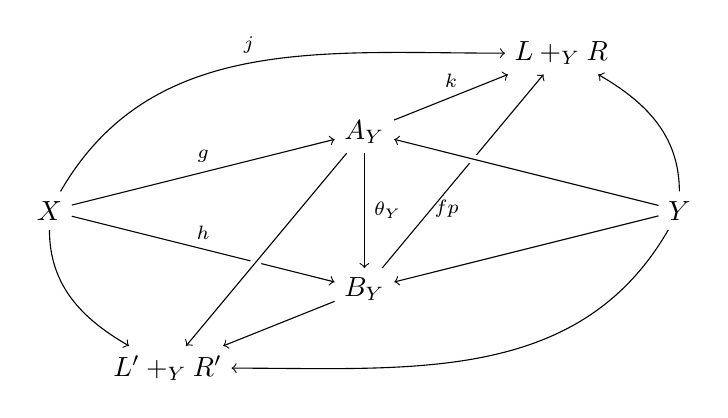
\begin{tikzpicture}
\node (X) at (-4,0) {$X$};
\node (LyR) at (2.5,2) {$L+_YR$};
\node (Y) at (4,0) {$Y$};
\node (LyR') at (-2.5,-2) {$L'+_YR'$};
\node (Ay) at (0,1) {$A_Y$};
\node (By) at (0,-1) {$B_Y$};
%
\draw [font=\scriptsize,->] (X) edge[in=180,out=60] node[above] {$j$} (LyR);
\draw [font=\scriptsize,->] (X) edge node[above] {$g$} (Ay);
\draw [font=\scriptsize,->] (X) edge node[above] {$h$} (By);
\draw [->] (X) edge[out=-90,in=150] (LyR');
\draw [->] (Y) edge[out=90,in=-30] (LyR);
\draw [->] (Y) edge[] (By);
\draw [->] (Y) edge[out=-120,in=0] (LyR');
\draw [font=\scriptsize,->] (Ay) edge node[above] {$k$} (LyR);
\draw [font=\scriptsize,->] (Ay) edge node[right] {$\theta_Y$} (By);
\draw [font=\scriptsize,->] (By) edge[pos=0.4] node[below] {$fp$} (LyR);
\draw [->] (By) edge[] (LyR');
%
\draw [->] (Y) edge[white,line width=3.5pt] (Ay);
\draw [->] (Y) edge[] (Ay);
\draw [->] (Ay) edge[white,line width=3.5pt] (LyR');
\draw [->] (Ay) edge[] (LyR');
\end{tikzpicture}
\]
\end{document}
